 % !TEX root = Stanfill_CoDA.tex
\section{Simulation Study}\label{ch:simulation}

Section~\ref{subsec:simdesign} gives an outline of the simulation design.  Section~\ref{subsec:genRR} briefly describes the parametric distributional models for describing symmetric rotation errors (cf.~(\ref{eqn:1})) of differing variability used in the study. 
\subsection{Design of Simulation Study}
\label{subsec:simdesign}
To compare the performance of the proposed location estimators for determining the central direction $\bm{S}$ given a sample of size $n$, we generated random rotation error samples  $\bm E_1, \ldots, \bm E_n$  in model \eqref{eqn:1} with sizes $n=10, 50, 100$ and 300. In \eqref{eqn:1}, without loss of generality, we set the location parameter $\bm S=\bm I_{3\times 3}$ (the identity matrix). To compare the performance of the estimators for different probability models for random rotations exhibiting the same spread, % we choose the circular variance defined as $\nu=1-\mathrm{E}[\cos(r)]$ as a measure %of spread for the circular densities of the angle $r$. Note that $\mathrm{E}[\cos(r)]$ is %commonly referred to as the mean resultant length. 
we consider varying circular variances $\nu=0.25$, $0.50$ and $0.75$ (described in Section~\ref{subsec:genRR}). For each combination of sample size, $\nu$ and choice of distribution, we generated 1,000 samples and for each sample estimated the central direction  $\bm S=\bm I_{3\times 3}$ using each of the four proposed estimators.  We continue with an introduction to the considered distributions for rotations in the next section.

%\red{that is  a bit abrupt -- should we move all of the above discussion relating to the densities to the next subsection? HH}
%For each combination of sample size, circular spread $\nu$ and choice of distribution, we generated 1,000 samples and for each sample estimated the central direction  $\bm S=\bm I_{3\times 3}$ using each of the four proposed estimators.  We continue with an introduction to the distributions under consideration in the next section.


\subsection{Generating Random Rotations in the Location Model}
\label{subsec:genRR}
%As mentioned in the introduction, 
We wish to compare estimators of the (fixed) location parameter $\bm{S}\in SO(3)$ under three common distributional models for describing symmetric rotation errors $\bm{E}\in SO(3)$ in a data model  $\bm{R}=\bm{S}\bm{E}$ (cf.~(\ref{eqn:1})): the symmetric matrix Fisher \citep{langevin05, downs72, khatri77, jupp79}, the symmetric Cayley  \citep{Schaeben97, leon06} and the circular-von Mises-based distribution \citep{bingham09}. A general construction approach exists for random rotations that are symmetrically distributed around the identity matrix $\bm{I}_{3 \times 3}$; see \cite{watson83, bingham09} and \cite{hielscher10}.  To this end, let $\bm{U}\in\mathbb{R}^3$ represent a point chosen uniformly on the unit sphere and, independently, generate a random angle $r$ according to some circular density $C(r|\kappa)$ on $(-\pi,\pi]$, which is symmetric around 0 and where $\kappa$ denotes a concentration parameter governing the spread of the circular distribution.  Then, define a random rotation as $\bm{E}=\bm{E}(\bm{U},r)$ using the constructive definition (\ref{eqn:angleaxis}) (i.e., $\bm{E}$ represents the position of $\bm{I}_{3\times 3}$ upon rotating the standard coordinate frame in $\mathbb{R}^3$ about the random axis $\bm{U}$ by the random angle $r$). The resulting rotation $\bm{E}$ will be symmetrically distributed and its distributional type (i.e., matrix Fisher, Cayley or circular-von Mises-based) is determined by the form of the circular density $C(r|\kappa)$ for the (misorientation) angle $r$. The circular densities  for the three distributions on rotations above are given in Table~\ref{tab:ang.dens}, where $\mathrm{I_p}(\cdot)$ denotes the Bessel function of order $p$ defined as  $\mathrm{I_p}(\kappa)=\frac{1}{2\pi}\int_{-\pi}^{\pi}\cos(pr)e^{\kappa\cos r}dr$.  The variability in the density $C(r|\kappa)$ of the angle $r$ controls the variability in the resulting constructed rotations and, for consistency, we use the circular variance defined as $\nu=1-\rho$ as a measure of spread for the circular densities for $r$ in Table~\ref{tab:ang.dens}. (Note that $\mathrm{E}[\cos(r)]$ is commonly referred to as the mean resultant length.) The values of $\kappa$ corresponding to the chosen circular variances $\nu$ are given in Table~\ref{tab:kappas}.

%To ease the interpretation of the simulation results in Section~\ref{sec:results},  we choose not to present results in terms of $\kappa$ but instead use the circular variance defined as $\nu=1-\rho$ as a measure of spread, where $\rho=\mathrm{E}[\cos(r)]$, which is commonly referred to as the mean resultant length. This allows us to compare the performance of the estimators for densities exhibiting the same spread.  The values of $\kappa$ corresponding to the chosen circular variances are given in Table~\ref{tab:kappas}.

%\begin{center} 
\begin{table}[h!]
\caption{Circular densities with respect to the Lebesgue measure and circular variance $\nu$.}  \label{tab:ang.dens}\centering
\small{
\begin{tabular}{ lclcl}\hline
\textbf{Name} & & \textbf{Density} $C(r |\kappa)$ & & \textbf{Circular variance $\nu$}\\ \hline \hline 
\rule[2mm]{0mm}{6mm} Cayley & & $\frac{1}
{\sqrt{\pi}} \frac{\Gamma(\kappa+2)}{\Gamma(\kappa+1/2)} 
2^{-(\kappa+1)} (1+\cos r)^\kappa(1-\cos r)$ & & $\frac{3}
{\kappa+2}$ \\
\rule[2mm]{0mm}{6mm} matrix Fisher & & $\frac{1}{2\pi[\mathrm{I_0}(2\kappa)-\mathrm{I_1}(2\kappa)]}e^{2\kappa 
\cos(r)}[1-\cos(r)]$ & & 
$\frac{3\mathrm{I}_0(2\kappa)-4\mathrm{I}_1(2\kappa)+\mathrm{I}_2(2\kappa)}
{2[\mathrm{I}_0(2\kappa)-\mathrm{I}_1(2\kappa)]}$ \\
\rule[2mm]{0mm}{6mm} circular-von Mises & & $\frac{1}{2\pi \mathrm{I_0}(\kappa)}e^{\kappa\cos(r)}$&  & 
$\frac{\mathrm{I_0}(\kappa)-\mathrm{I_1}(\kappa)}{\mathrm{I_0}(\kappa)}$ \\[-7mm] 
\rule[2mm]{0mm}{6mm} & & & & \\\hline
\end{tabular}}
\end{table}
%\end{center}

%\begin{center}
\begin{table}[h!]
\caption{Values of $\kappa$ for each rotational distribution corresponding to the circular variances.}  \label{tab:kappas}%\vspace{-0.4cm}
\centering
\begin{tabular}{l l ccc}\hline
{\bf Distribution} & & \multicolumn{3}{c}{\bf Circular variance $\nu$} \\
& & $0.25$ &$0.50$ & $0.75$\\ \hline \hline
Cayley & & 10.00 & 4.00 & 2.00 \\
matrix Fisher & & 3.17 & 1.71 & 1.15\\
circular-von Mises & & 2.40 & 1.16 & 0.52\\ \hline
\end{tabular}
\end{table}
%\end{center}

The density, with respect to the Haar measure, for each distribution of a random rotation given a circular variance of $0.75$ is plotted in Figure~\ref{fig:Haar}.  The Haar measure (or uniform distribution on $SO(3)$) acts as the dominating measure for rotations and the symmetric nature of the random rotation $\bm E_i=\bm E_i(\bm U,r)$ means that its density $f(\bm E_i|\nu)=f(r|\nu)$ can be plotted in terms of the misorientation angle $r$ of $\bm E_i$ in \eqref{eqn:angleaxis}, which is common in materials science \citep{matthies88, savyolova95}.  Density plots with the other circular variances  considered in our simulations  are similar.

%Old figures the AE didn't like.  Wanted us to show whole c-vM distribution and add zoom plot here to save space.
% \begin{figure}[h!]
% \centering
% \subfloat[$\nu=0.25$]{\label{fig:cayden}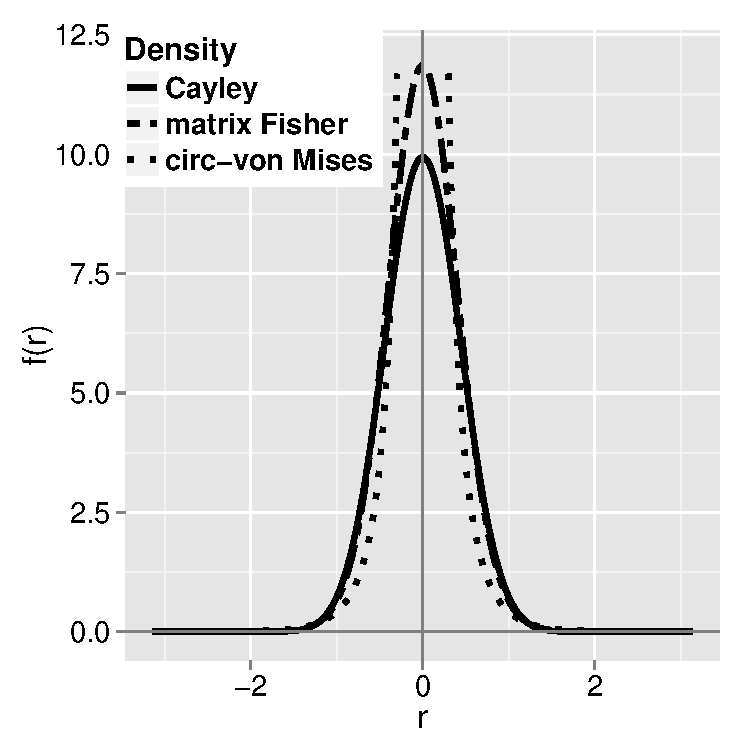
\includegraphics[width=0.33\textwidth]{Var25DensityHaar.pdf}}
% \subfloat[$\nu=0.50$]{\label{fig:fishden}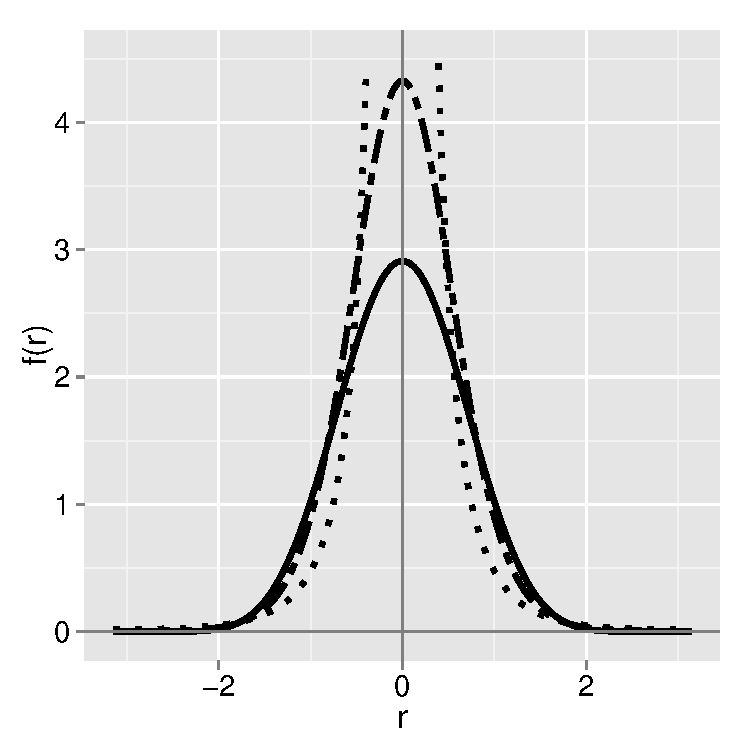
\includegraphics[width=0.33\textwidth]{Var5DensityHaar.pdf}}
% \subfloat[$\nu=0.75$]{\label{fig:vonmden}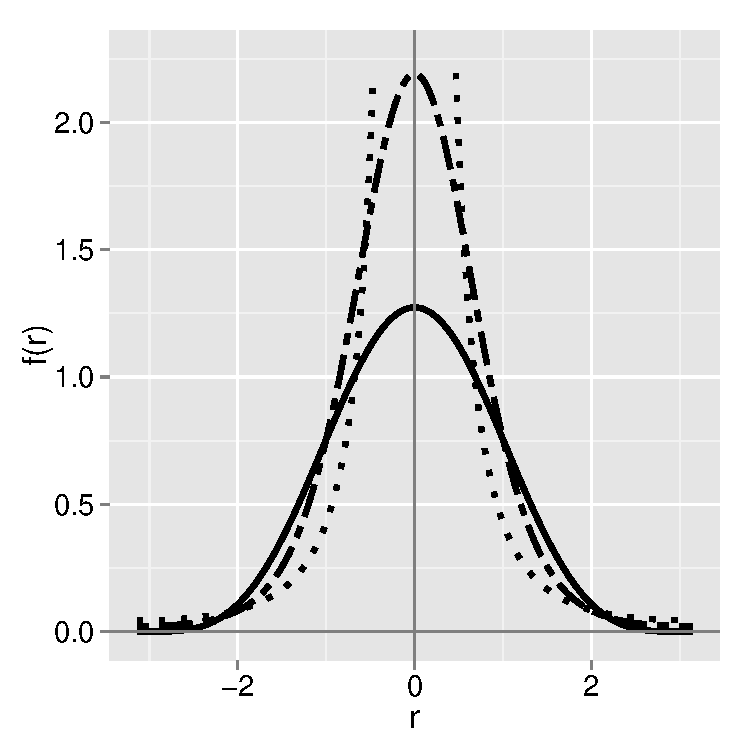
\includegraphics[width=0.33\textwidth]{Var75DensityHaar.pdf}}
% \caption{Density functions for the three rotational distributions with respect to the Haar measure. The solid line corresponds to the density of matrix Fisher distribution, the dashed line the density of the circular-von Mises-based distribution and the dotted line to the density of the Cayley distribution.}
% \label{fig:Haar}
% \end{figure}

\begin{figure}[h!]
\centering
\subfloat[Overview]{\label{fig:zoomout}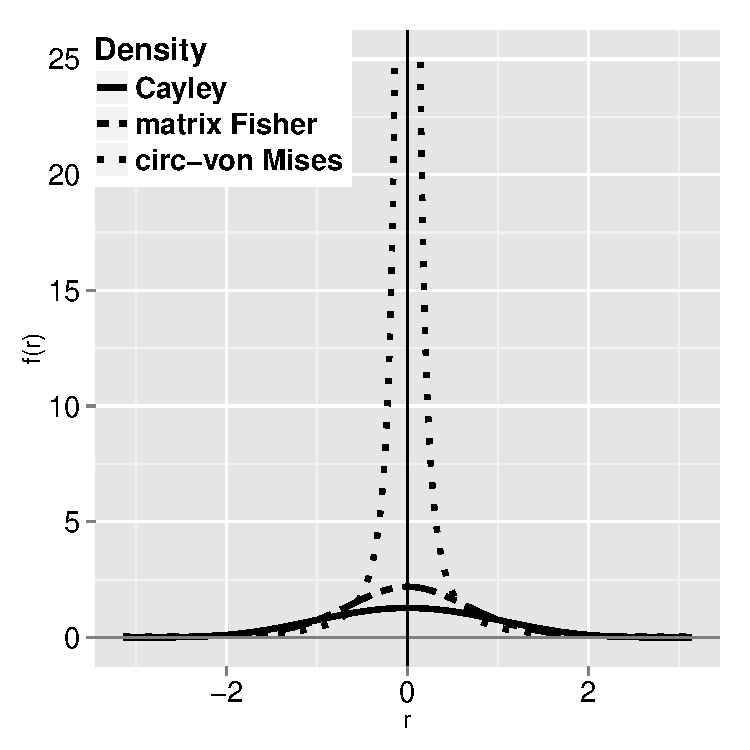
\includegraphics[width=0.33\textwidth]{Var75DensityHaarFull.pdf}}
\subfloat[Mode Behavior]{\label{fig:body}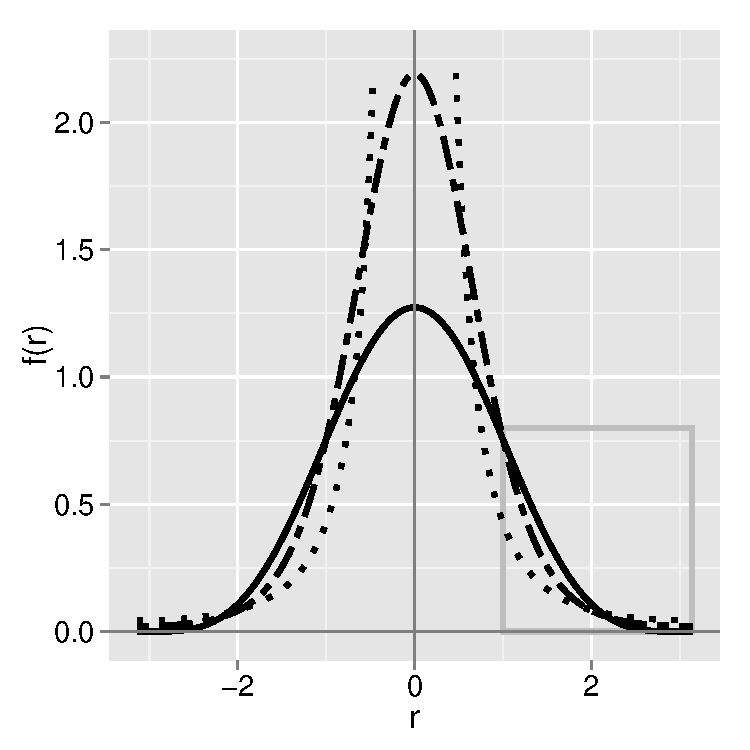
\includegraphics[width=0.33\textwidth]{Var75DensityBox.pdf}}
\subfloat[Tail Behavior]{\label{fig:denzoom}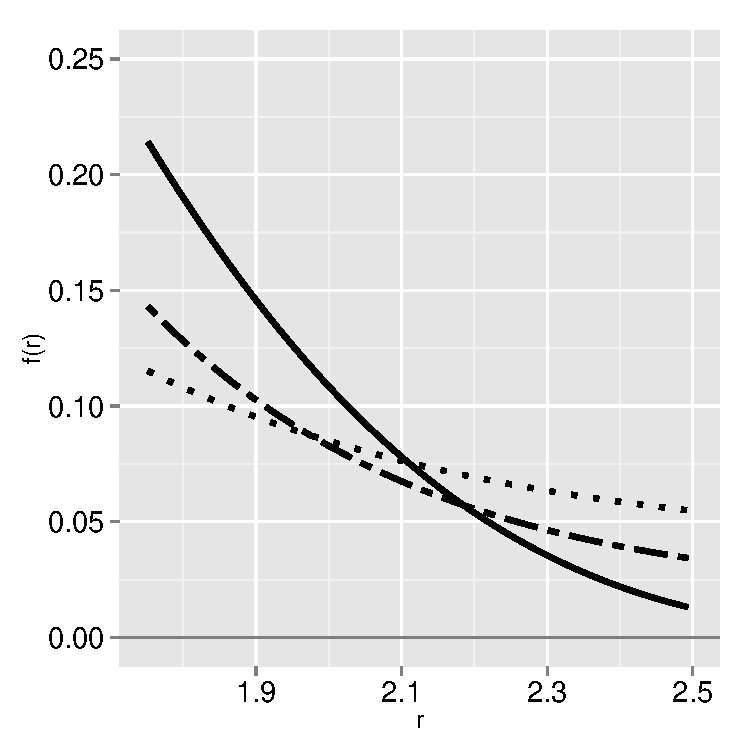
\includegraphics[width=0.33\textwidth]{Var75DensityZoomNoGuide.pdf}}
\caption{Density comparison for rotation distributions with $\nu=0.75$.  The circular-von Mises based-distribution has the highest concentration, but also the heaviest tail.}
\label{fig:Haar}
\end{figure}

In Figure~\ref{fig:Haar}(a)-(b), we see that the circular-von Mises-based distribution has the most mass around the mode of zero whereas the Cayley distribution has the least mass around its mode.   Figure \ref{fig:Haar}(c) offers a better view of the tail behavior of the distributions. 
A visualization of a random sample of 100 rotations, one sample for each of the three angular distributions, is given in the sphere plots in Figure~\ref{eyeballs}. The samples are adjusted to have an circular variance of $\nu = 0.25$.  Note that Figure~\ref{eyeballs} shows only the first of the three columns of each rotation matrix. We refer to the supplemental material online for a complete visualization of the three samples.
%Section~\ref{sec:appendix.eyeballs} 
\begin{figure}[htbp]
\centering
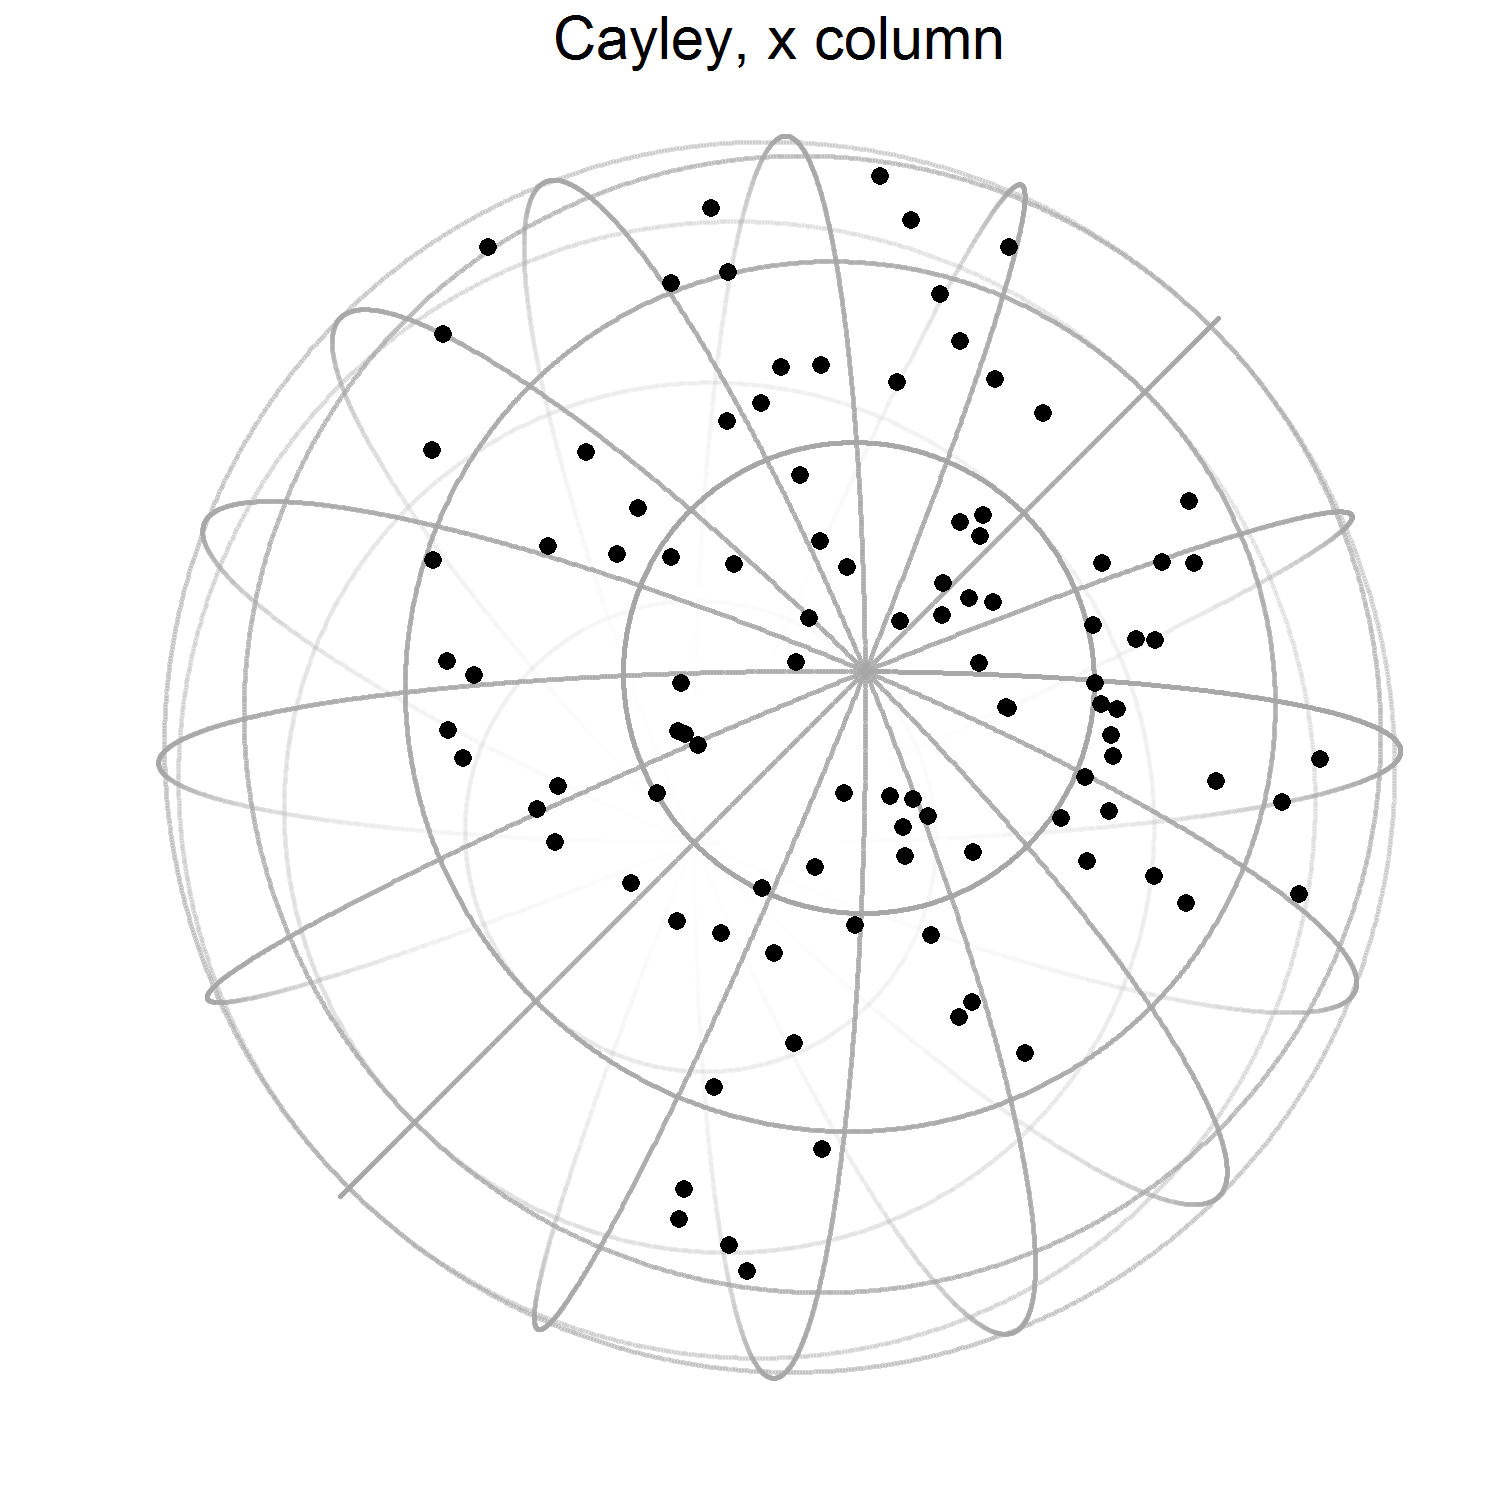
\includegraphics[width=.3\linewidth]{eye-cayley}
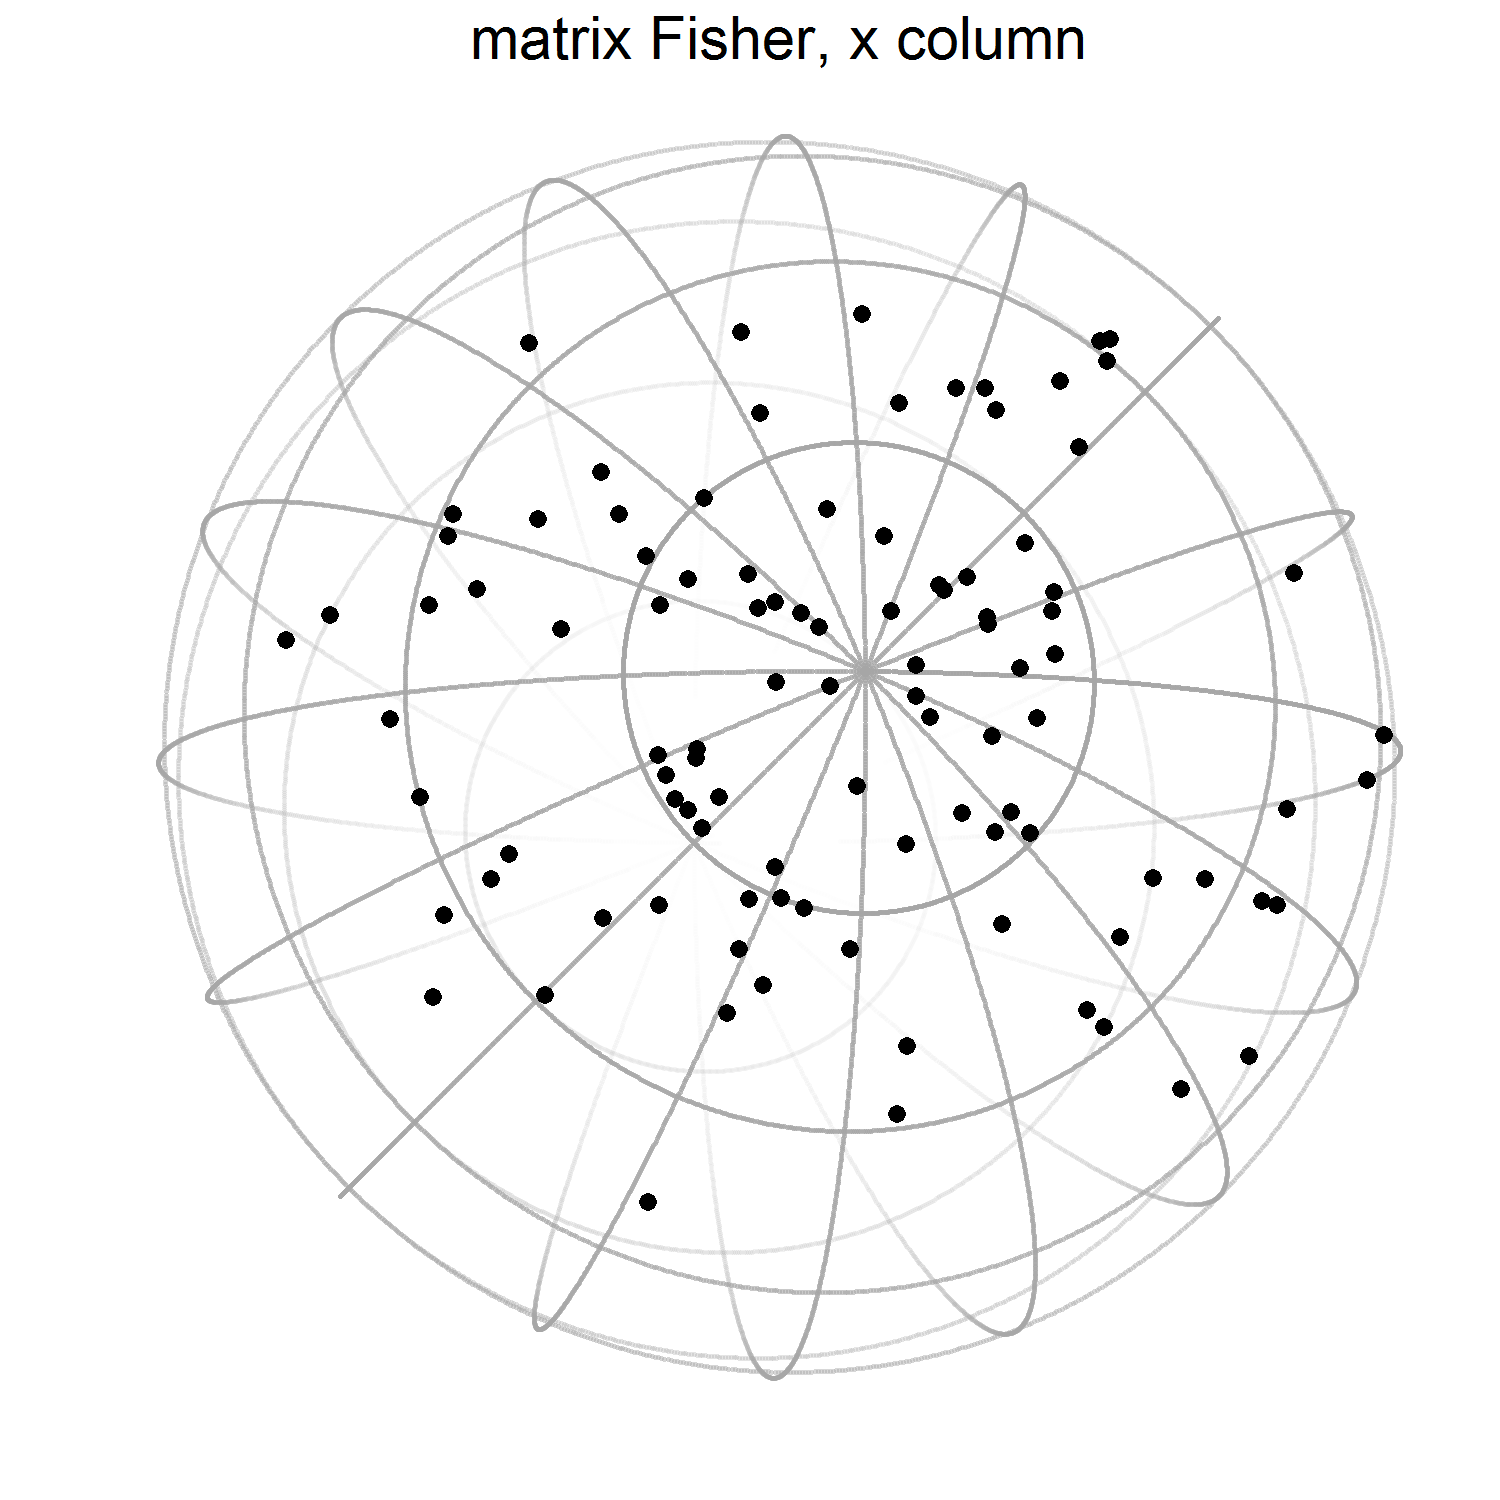
\includegraphics[width=.3\linewidth]{eye-fisher}
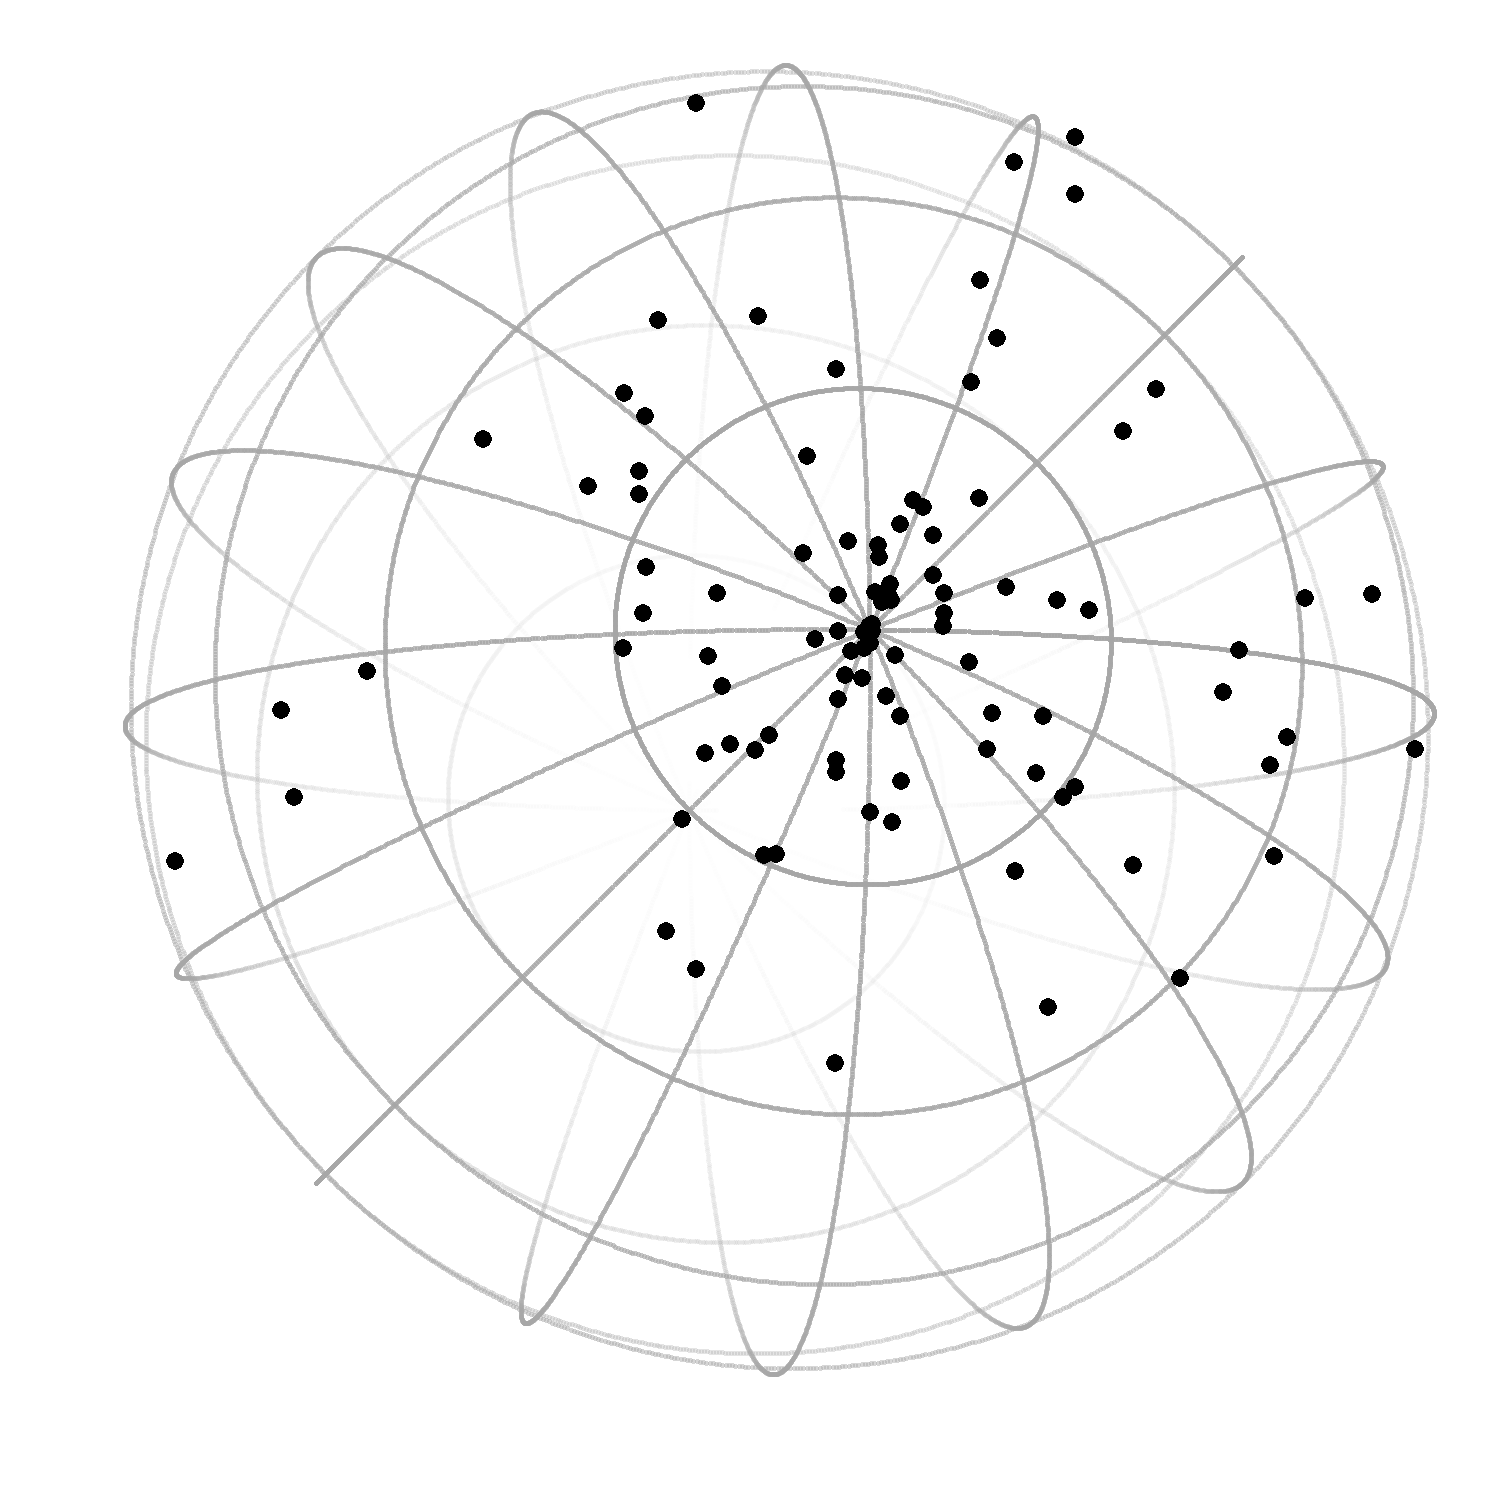
\includegraphics[width=.3\linewidth]{eye-vmises}
\caption{\label{eyeballs}Sphere plots of the first column for randomly generated rotations with different distributions having  $\nu = 0.25$}
\end{figure}
In the simulation study to follow, for generating random rotation errors based on the construction above, we used different samplers to randomly generate angles $r\in(-\pi,\pi]$ from a given circular density, recalling that the form of $C(r|\kappa)$ depends on the intended symmetric distribution for the rotation errors $\bm{E}$, see also the supplemental material on-line.

%\subsection{Estimator Algorithms}
%\label{subsec:algorithms}

%Two of the estimators of interest require a projection from the space of all $3\times 3$ matrices, $\mathcal{M}(3)$, into $SO(3)$.  We perform this projection according to the following method.  For a matrix $\bm M\in\mathcal{M}(3)$ let $\lambda_1 \geq \lambda_2 \geq \lambda_3$ denote the ordered eigenvalues of $\bm M^\top\bm M$ with corresponding eigenvectors $ \bm u_1, \bm u_2, \bm u_3$.  Defining $\bm U=[\bm u_1, \bm u_2, \bm u_3]$ and provided that $\det(\bm M)\neq 0$, the unique projection of $\bm M$ into $SO(3)$ is given by
%\[
%\bm M\bm{U} \text{diag}\left(\frac{1}{\sqrt{\lambda_1}},\frac{1}{\sqrt{\lambda_2}},\frac{\text{sign}\left[\det(\bm M)\right]}{\sqrt{\lambda_3}}\right) \bm{U}^\top.
%\]
%We will refer to this as the $\mathcal{M}(3)$ projection algorithm. To calculate $\widehat{\bm{S}}_P$ given a sample $\{\bm{R}_1,\dots,\bm{R}_n\}\subset SO(3)$ we compute the $\mathcal{M}(3)$ projection of $\bar{\bm R}=\frac{1}{n}\sum_{i=1}^n\bm{R}_i$.  See \citet{arun87,horn88} and \citet{umeyama91} for an introduction and refinements of this solution including special cases such as $\det(\bar{\bm R})=0$.

%To compute the projected median $\widetilde{\bm S}_P$ we use a Weiszfeld-type algorithm originally given by \cite{weiszfeld37}.  The algorithm requires an initial value that does not equal any sample point. For the purpose of speeding up computing time we use $\widehat{\bm S}_P$ as the starting point. Note that the solution is generally not sensitive to the choice of starting points unless the data exhibit extreme spread.
%\begin{enumerate}
%\item Set $\widehat{\bm S}=\widehat{\bm S}_{P}$ and choose an arbitrarily small stopping rule $\varepsilon$.
%\item For $i=1,\ldots,n$ compute $\bm s_i=\bm R_i-\widehat{\bm S}$.
%\item Calculate
%\[
%\bar{\bm R}_W=\frac{\sum_{i=1}^n\bm R_i/||\bm s_i||_F}{\sum_{i=1}^n1/||\bm s_i||_F}
%\]
%which we call the weighted mean with respect to $\widehat{\bm S}$.
%\item Define $\widehat{\bm S}_{\text{new}}$ to be the $\mathcal{M}(3)$ projection of $\bar{\bm R}_W$.
%\item If $\varepsilon>||\widehat{\bm S}-\widehat{\bm S}_{\text{new}}||_F$ return $\widetilde{\bm{S}}_P=\widehat{\bm S}_{\text{new}}$; otherwise set $\widehat{\bm S}=\widehat{\bm S}_{\text{new}}$ and return to step 2.
%\end{enumerate}

%The second set of algorithms is based on the relationship between $SO(3)$ and its tangent space $\mathfrak{so}(3)$ through the principal logarithm of a rotation $\bm R$, see Sections~\ref{subsec:geometry} and \ref{subsec:metrics}. The rotation that minimizes the sum of the squared geodesic distances, $\widehat{\bm S}_G$, for a given tolerance level $\varepsilon$ can be found as follows \citep[see][]{manton04}.
%\begin{enumerate}
%\item Initiate a value for $\widehat{\bm S}$, e.g. $\widehat{\bm S}= \widehat{\bm S}_P$ .
%\item Calculate $\bm s=\frac{1}{n}\sum_{i=1}^n\Log(\widehat{\bm{S}}^\top\bm R_i)$.
%\item If $||\bm s||_F<\varepsilon$ return $\widehat{\bm S}_{G}=\widehat{\bm S}$; otherwise set $\widehat{\bm S}=\widehat{\bm S}\exp(\bm s)$ (see Section~\ref{subsec:geometry}), repeat step 2 and re-evaluate.
%\end{enumerate}


%Finally, to find the minimizer of the first order geodesic distances we use an algorithm developed by \citet{hartley11}.  Similar to $\widetilde{\bm S}_{P}$, this algorithm requires a starting point not in the sample, so we use $\widehat{\bm S}_{G}$ to save computational time.
%\begin{enumerate}
%\item Set $\widehat{\bm S}=\widehat{\bm S}_{G}$.
%\item For each sample point compute $\bm s_i=\Log(\widehat{\bm S}^\top\bm R_i)$.
%\item Set 
%\[
%\bm\delta=\frac{\sum_{i=1}^n \bm s_i/||\bm s_i||_F}{\sum_{i=1}^n 1/||\bm s_i||_F}.
%\]
%\item If $||\bm\delta||_F<\varepsilon$ then return $\widetilde{\bm S}_{G}=\widehat{\bm S}$; otherwise update $\widehat{\bm S}=\exp(\bm\delta)\widehat{\bm S}$ and return to step 2.
%\end{enumerate}

